
\chapter{Ultrafast Structural Dynamics of (EDO-TTF)\textsubscript{2}X}
\label{ch: UED-EDO}

In this chapter, I will present two studies on the photoinduced structural dynamics
of the crystalline material (EDO-TTF)\textsubscript{2}X. For context,
a general overview of this molecular system will be given. This is followed by a description
of the experimental procedure and a discussion of the results from the studies.
The works herein have been reported in the articles
``Mapping Molecular Motions Leading to Charge Delocalization with Ultrabright Electrons''
and ``Ultrafast Electron Diffraction Study of Single-Crystal
(EDO-TTF)\textsubscript{2}SbF\textsubscript{6}: Counterion Effect and Dimensionality Reduction,''
previously published in the journals Nature and Chemical Physics Letters respectively~\cite{Gao2013, Liu2017}.

\section{Overview of (EDO-TTF)\textsubscript{2}X Molecular Systems}
\label{sec: UED-EDO-overview}

In 1941, Albert Szent-Gy\"{o}rgyi%
\footnote{Albert Szent-Gy\"{o}rgyi (1893--1986) is a Hungarian biochemist
who won the Nobel Prize in Physiology or Medicine in 1937
for his work in vitamin C and the chemistry of cellular respiration~\cite{Nobel1922}.}%
proposed that some processes in biological systems, such as photosynthesis,
could be explained by long-range light-induced transfer of electrons
through a chain of interacting proteins in a manner analogous to electrical conduction in metals
as described by band theory~\cite{Szent1941, Szent1946}.
%
Such an `organic metal' would combine the mechanical and functional versatility of an organic%
\footnote{`Organic' originally refers to that which is solely derived from living organisms;
it has now been generalized to describe chemistry that involves the element carbon,
often in association with other nonmetals.}
compound with the electron transport properties of a conventional metal ($\sigma \gtrsim 10^3$~S/cm,
see Fig.~\ref{fig: EDO-overview}a).
%
\begin{figure}[ht!]
  \centering
  \includegraphics[width = \textwidth]{Figures/fig_EDO_overview.pdf}
  \caption[Overview of organic metallicity.]{
  Overview of organic metallicity.
  (a) Electrical conductivity of various materials for comparison~\cite{CRCHandbook, TTFBook}.
  (b) Structural building blocks of Bechgaard-Fabre salts and related compounds
  (white = hydrogen, black = carbon, blue = nitrogen, red = oxygen, green = fluorine, brown = phosphorus, orange = selenium).
  (c) Schematic of the crystal structure of (TMTSF)\textsubscript{2}PF\textsubscript{6},
  showing the overlapping regions of positive (pink) and negative (gray) charge
  that enable electrical conduction.
  (d) Generalized phase diagram of Bechgaard-Fabre salts;
  behaviour at standard ambient pressure is indicated by arrows at top;
  abbreviations: `loc' = localization, `CO' = charge ordering, `SP' = spin-Peierls,
  `AFM' = antiferromagnetism, `SDW' = spin-density wave, `SC' = superconductivity, `ND' = n-dimensional;
  solid lines represent phase transitions while dashed lines are crossovers.
  (e) Electrical resistivity $\rho_\parallel$ along the stacking axis
  as a function of temperature at standard ambient pressure;
  note the superconductive transition of (TMTSF)\textsubscript{2}ClO\textsubscript{4}.
  Panels~(c)--(e) are adapted with permission from
  Refs.~\cite{BechgaardJerome1982, Dressel2007, Jerome1982} respectively.
  }
  \label{fig: EDO-overview}
\end{figure}
%
This prospect stimulated significant interest amongst chemists and material scientists,
leading to the discovery of moderately conductive but short-lived compounds like perylene--bromine
($\sigma \sim 1$~S/cm) in 1954~\cite{Akamatu1954} and a proposal by William A. Lamb in 1964
of a synthetic organic polymer that remains superconductive at room temperature~\cite{Little1964}.

A major breakthrough came in 1977 when Shirakawa and his collaborators%
\footnote{This work netted the 2000 Nobel Prize in Chemistry
for Alan J. Heeger (1936--present), Alan G. MacDiarmid (1927--2007),
and Hideki Shirakawa (1936--present)~\cite{Nobel1996}.}
%
discovered that doping \textit{trans}-polyacetylene with iodine vapour
can increase its electrical conductivity by seven orders of magnitude,
reaching $\sigma = 38$~S/cm at room temperature~\cite{Shirakawa1977}.
Around the same time, Coleman, Ferraris, and their coworkers combined
two recently discovered molecules, tetrathiafulvalene~(TTF) and
tetracyano-\textit{p}-quinodimethane~(TCNQ),
to prepare a 1:1 complex that, when crystallized,
conducts like a metal over a large range of temperature
($\sigma_\text{max} = 1.47 \times 10^4$~S/cm)~\cite{Wudl1970, Coleman1973, Ferraris1973}.

The molecule TTF-TCNQ was not simply the result of serendipity but a sagacious feat of molecular design.
%
High electron mobility requires good overlap of valence orbitals
that are not completely filled, thus allowing electrons to easily move from one molecule to another.
However, this requirement also tends to destabilize the material
as the unpaired valence electrons make it susceptible to chemical attack by other substances.
%
It happens that TTF and TCNQ can readily donate and accept electrons
while remaining chemically stable because of the aromaticity%
\footnote{A molecule is said to be aromatic when it has a flat ring of atoms
bound together by an set of overlapping p orbitals.}
of the resulting radical ions, TTF$^+$ and TCNQ$^-$~\cite{LittleBook}.

When crystallized together, TTF and TCNQ molecules self-assemble into
separate stacks of molecules lying parallel to each other
as each species interacts amongst themselves through their heteroatoms and
$\unslant[-.2]\pi$~orbitals (see Fig.~\ref{fig: EDO-overview}b).
%
A partial charge transfer (ca.~$0.56$~e$^-$) occurs and the ions flatten,
further overlapping the $\unslant[-.2]\pi$ orbitals within each stack and
forming an array of conductive wires through the crystal
in the direction of the stacking axis.

In the absence of significant interstack orbital overlap,
bulk TTF-TCNQ behaves as a loose ensemble of
quasi-one-dimensional electron systems, which are highly susceptible to
Peierls instability,%
\footnote{Rudolf E. Peierls (1907--1995) noted in 1954 that
one-dimensional periodic arrangements of atoms with delocalized electrons
tend to dimerize due to electron--phonon coupling~\cite{PeierlsBook}.
}
%
a cooperative phenomenon that eventually destroys the conductive state of TTF-TCNQ
at low temperature ($T \approx $~38--54~K).
%
In a bid to stave off this metal--insulator~(MI) phase transition,
Bechgaard, Fabre, and their coworkers synthesized a new class of
charge-transfer~(CT) compounds based on molecular design principles
similar to those of TTF-TCNQ~\cite{Bechgaard1980}.
%
Known as Bechgaard-Fabre salts,%
\footnote{Named for Danish chemist Klaus Bechgaard (1945--2017) and
French chemist Jean-Marc Fabre (1943--present) who respectively
first synthesized the selenium (TMTSF) and sulfur (TMTTF) derivatives of TMTCF~\cite{Pouget2012}.}
%
they have the chemical formula (TMTCF)\textsubscript{2}X,
where TMTCF$^{0.5+}$ is tetramethyl-tetrachalcofulvalene
and X is a monovalent weakly-coordinating anion like
hexafluoropnictate (PnF\textsubscript{6}$^-$).%
\footnote{Chalcogens are chemical elements in group 16 of the periodic table, e.g.~sulfur and selenium;
pnictogens are those in group 15, e.g.~phosphorus and antimony.}

When crystallized, (TMTCF)\textsubscript{2}X forms a strongly anisotropic material
as the flat cations assemble in parallel, into conductive stacks separated by columns of isolated anions
(see Fig.~\ref{fig: EDO-overview}c for a schematic view).
%
Given this lattice structure and the resulting electronic system,
competing interactions and a subtle interplay
of the charge, spin, and nuclear degrees of freedom
give rise to a variety of collective phenomena~\cite{Kohler2011}.
%
In Fig.~\ref{fig: EDO-overview}d,
a generalized phase diagram of Bechgaard-Fabre salts is shown;
it is replete with ground states separated by phase transitions and crossovers
that can be induced by fine-tuning the coupling within and between the molecular stacks
through pressure --- externally applied
or chemically induced via anion substitution~\cite{Jerome1991}.
%
In 1980, it was discovered that superconductivity could be achieved in
(TMTSF)\textsubscript{2}PF\textsubscript{6} at $T \leq 1.3$~K
by applying $>6$~kBar of pressure~\cite{Bechgaard1980, Jerome1980};
one year later, the perchlorate (ClO\textsubscript{4}$^-$) salt was found
to become superconductive at about the same temperature but under standard ambient pressure
(Fig.~\ref{fig: EDO-overview}e)~\cite{Bechgaard1981, Jerome1982}.

From above, it is clear that the material properties of Bechgaard-Fabre salts depend crucially on
the network of orbital overlaps and weak intermolecular interactions throughout the crystal lattice.
%
To explore this rich physics, numerous other derivatives of prototypical TTF~molecule have been synthesized
by attaching functional substituents to both or either side of the TTF~core.
%
One of them is 4,5-ethylenedioxy-tetrathiafulvalene (EDO-TTF)~\cite{Papavassiliou1990, Mori1990, Meziere2000}
and its 2:1 radical-cation salts (EDO-TTF)\textsubscript{2}X
have been observed to exhibit a MI phase transition upon cooling
unlike any other before~\cite{Ota2002, Ota2003, Ota2006}.

\begin{figure}[ht!]
  \centering
  \includegraphics[width = \textwidth]{Figures/fig_EDO_static.pdf}
  \caption[Metal--insulator phase transition in (EDO-TTF)\textsubscript{2}PF\textsubscript{6}.]{
  Metal--insulator phase transition in (EDO-TTF)\textsubscript{2}PF\textsubscript{6}.
  Temperature dependence of (a) electrical resistivity, (b) magnetic susceptibility,
  and (c) optical conductivity along the stacking axis.
  (d) Raman spectra of (EDO-TTF)\textsubscript{2}AsF\textsubscript{6}
  above and below $T_\text{MI}$, along with that of neutral EDO-TTF and
  (EDO-TTF)$^+$(IBr\textsubscript{2})$^-$;
  peaks associated with charge-sensitive C=C stretching modes are color-coded.
  Charge density isosurfaces (0.7~e$^-$/\AA$^3$) calculated from XRD data,
  as viewed (e) along the stacking axis and (f) from the side,
  coloured by charge state (blue: $+1e$, green: $+0.5e$, yellow: $+0e$, red: $-1e$);
  (g) lower isosurfaces (ca.~$0.1$~e$^-$/\AA$^3$)
  with relevant orbital overlap integral values $S$ ($\times 10^{-3}$).
  (h) Thermal ellipsoids of the PF\textsubscript{6} anions.
  Panels~(a), (b), and (g) are adapted with permission from Ref.~\cite{Ota2002};
  (c) and (d), from Refs.~\cite{Drozdova2003, Drozdova2004} respectively;
  (e)--(f), from Ref.~\cite{Aoyagi2004}.
  }
  \label{fig: EDO-static}
\end{figure}
%
At room temperature, single-crystal (EDO-TTF)\textsubscript{2}PF\textsubscript{6}
appears black and is highly reflective.
%
As seen in Fig.~\ref{fig: EDO-static}a,
the electrical conductivity decreases abruptly at $279.0$~K from $60$~S/cm to
$1.4 \times 10^{-5}$~S/cm and subsequently varies with an activation energy of $0.52$~eV,
indicating a first-order MI phase transition from a high-temperature (HT) metallic phase
to a low-temperature (LT) insulator phase at $T_\text{MI} = 279.0$~K.
%
This is observed again with optical conductivity measurements (Fig.~\ref{fig: EDO-static}c),
which show the simultaneous disappearance of a broad Drude%
\footnote{German physicist Paul Drude (1863--1906) studied optical phenomena
from the perspective of electromagnetism and introduced a classical model of metals
to explain their transport properties~\cite{DrudeBioBook}.}
feature typical of metals and the appearance of two sharp peaks at 4500~cm$^{-1}$ and 11150~cm$^{-1}$.

XRD measurements of the HT phase reveal a triclinic crystal structure with P$\overline{1}$ symmetry,
not too dissimilar to those of (TMTCF)\textsubscript{2}X:
`nearly flat' EDO-TTF molecules stacked perpendicularly in a head--tail arrangement
with PF\textsubscript{6} molecules at cell vertices,
slotted in the soft cavities formed by the terminal ethylene groups.
Overlapping $\unslant[-.2]\pi$~orbitals along the stacking axis form
a quasi-1D electronic band structure that becomes $\frac{3}{4}$-filled%
\footnote{Hole-wise, $\frac{1}{4}$-filled; each of the two EDO-TTF molecules has two valence electrons
and one of the four in total is transferred to the PF\textsubscript{6} molecule.}
during the CT process.
%
The LT phase has a significantly different crystal structure:
the P$\overline{1}$ triclinic unit cell is doubled along the stacking axis
to include four EDO-TTF molecules,
alternating pairwise between two nonequivalent --- `flat' and `bent'%
\footnote{The curvature of the EDO-TTF molecule refers to the sum of
the dihedral angles of the atom chain O--C--S--C and C=C--S--C;
`flat': 1.87$^\circ$, `nearly flat': 2.08$^\circ$, `bent': 13.42$^\circ$.} ---
structures and two PF\textsubscript{6} molecules that are displaced from
the highly symmetric cell vertices.
%
These concomitant pairwise symmetry-breaking structural distortions indicates that
the MI phase transition is in part driven by Peierls instability.
This cooperativity is also evidenced by the bistability of phases seen in
the thermal hysteresis of the magnetic susceptibility (Fig.~\ref{fig: EDO-static}b).

Close inspection of the charge density reconstructed from the XRD data reveals
other unexpected differences between the LT and HT phases.
As seen in Fig.~\ref{fig: EDO-static}g, a `bond order' is apparent
when the intermolecular distances and orbital overlap integral values are calculated~\cite{Aoyagi2004};
below $T_\text{MI}$, bonding along the EDO-TTF stack strengthens
between the pairs of flat molecules while it weakens between the bent ones and
disappears between the dimers.

Furthermore, there is `anion ordering'~\cite{Ota2002}.
From Fig.~\ref{fig: EDO-static}h,
the PF\textsubscript{6} anions in the metallic HT phase are located at the inversion centres
of the unit cell and exhibit rotational disorder whilst the fluorine atoms are isotropically distributed
with large thermal ellipsoids.
%
In the insulator LT phase, the anions are displaced
from their special position of symmetry in the direction of the EDO-TTF stacking axis
and become uniaxially oriented as the atomic displacement parameters of the fluorine atoms
are drastically reduced and the F--P--F bonds point to the sulfur atoms on the neighbouring EDO-TTF molecules.
%
This suggests that the counterions are not merely spectating the MI phase transition
but are actively affected by the bond-coupled Peierls-type phonons of the EDO-TTF cations
through electrostatic interactions~\cite{Aoyagi2004}.

In Fig.~\ref{fig: EDO-static}d,
Raman spectra of (EDO-TTF)\textsubscript{2}X taken at different temperatures show splitting and shifting
of peaks associated with C=C stretching modes that are sensitive to the molecular charge.
Comparison with the spectrum of neutral and charged molecules suggests that the LT phase is composed of
electron donors in two different charge states~\cite{Drozdova2004}.
%
Analysis of charge-sensitive bond lengths~\cite{Ota2002} and
electron counting using XRD-derived charge densities~\cite{Aoyagi2004} further assign
a charge state of +0.5 to the nearly flat EDO-TTF molecules of the HT phase and
$+1e$ and $+0e$ to the flat and bent molecules of the LT phase respectively.%
\footnote{More precisely, nearly flat: $+(0.6 \pm 0.1)e$,
flat: $+(0.8 \pm 0.1)e$, and bent: $+(0.2 \pm 0.1)e$~\cite{Aoyagi2004}.}
%
Hence, a `charge order' commensurate with the previously described bond order
emerges during the MI~phase transition
as the charge-distributed state --- denoted D$^{+0.5}$D$^{+0.5}$D$^{+0.5}$D$^{+0.5}$ or $(\frac{1}{2} \frac{1}{2} \frac{1}{2} \frac{1}{2})$ ---
that is present in the metallic HT phase undergoes disproportionation and molecular deformation at $T_\text{MI}$,
transforming into the charge-localized $(1001)$ state of the insulator LT phase
(Fig.~\ref{fig: EDO-static}e--f).

It is remarkable that the $(1001)$ state of the LT phase is stable
since intuition would have instead given way to an alternating Wigner-type%
\footnote{Hungarian physicist and Nobel laureate Eugene P. Wigner (1902--1995) predicted in 1934
that a free electron gas would crystallize in the limit of zero kinetic energy~\cite{Nobel1963, Wigner1934}.}
$(1010)$ charge state wherein on- and off-site Coulomb repulsion would have been minimized,
as in the case of other quasi-1D molecular systems like
(DI-DCNQI)\textsubscript{2}Ag and (TMTTF)\textsubscript{2}PF\textsubscript{6}~\cite{Seo1997, Hiraki1998, Chow2000}.
%
However, this simplistic assessment ignores the energetic contribution of charge-dependent molecular deformations
and localized electrostatic interactions between the EDO-TTF and PF\textsubscript{6} molecules.
%
Indeed, the $(1001)$ charge order can be found when intermolecular Peierls-type and
intramolecular Holstein-type electron--phonon interactions are included in an extended Hubbard model%
\footnote{American physicist Theodore D. Holstein (1915--1985)~\cite{Emin1986}
introduced in a series of papers~\cite{Holstein1959} an eponymous electron--phonon coupling Hamiltonian
that describes electrons hopping around a fixed lattice of local oscillators;
British physicist John Hubbard (1931--1980)~\cite{Rice1981} also introduced
around the same time~\cite{Hubbard1963} a now-classic Hamiltonian that models
a system of hopping electrons that experience short- (on-site) and
intermediate- (nearest-neighbour) range Coulomb repulsion.}~\cite{Ung1994, Clay2003, Yonemitsu2007}.

Calculations using the `extended Peierls-Holstein-Hubbard' (ex-PHH) model Hamiltonian
(see App.~\ref{ap: exPHH})
have been used to reproduce and assign the two distinct peaks
--- 4500~cm$^{-1}$ ($= 0.56$~eV) and 11150~cm$^{-1}$ ($= 1.38$~eV) ---
in the optical conductivity spectrum of the LT phase (Fig.~\ref{fig: EDO-static}c).
%
Both%
\footnote{A third CT band (CT3) at 6150~cm$^{-1}$ ($= 0.76$~eV),
more clearly seen on shoulder of CT1 below 100~K, is assigned to an excitation
to a mixture of the $(1010)$ and $(2000)$ states~\cite{Drozdova2004}.}
appear to be charge-transfer bands (denoted CT1 and CT2),
resulting from electronic excitation of the type D$^+$D$^0$~$\rightarrow$~D$^0$D$^+$ or $(1001) \rightarrow (0101)$
and D$^+$D$^+$~$\rightarrow$~D$^{2+}$D$^0$ or $(1001) \rightarrow (2000)$
respectively~\cite{Drozdova2003, Drozdova2004, Yonemitsu2007}.
%
Given the close relationship between charge order and
the physics of the MI~phase transition of (EDO-TTF)\textsubscript{2}X,
these CT bands offer readily accessible pathways for controlling the physical properties of the material
via photoexcitation.
%
Earlier works on similar CT compounds suggested that so-called photoinduced phase transitions (PIPT)
can be triggered by pumping at their CT bands with ultrashort laser pulses~\cite{Koshihara1990, Karutz1998, Koshihara1998, Nasu2004}.


\begin{figure}[ht!]
  \centering
  \includegraphics[width = \textwidth]{Figures/fig_EDO_time-resolved.pdf}
  \caption[Ultrafast time-resolved pump-probe spectroscopy in
  (EDO-TTF)\textsubscript{2}PF\textsubscript{6}.]{
  (EDO-TTF)\textsubscript{2}PF\textsubscript{6} crystals at low temperature
  are studied with ultrafast time-resolved pump-probe spectroscopy
  using a $800$-nm $120$-fs pump and different probes.
  (a)~With photons spanning the CT2~band, a collapse in reflectivity was observed,
  indicating photoinduced metallization of the insulator LT phase within a few hundred femtoseconds.
  (b)~With a broadband near-IR probe, the transient optical conductivity spectrum was reconstructed,
  enabling its assignment to a $(1010)$-type electronic state.
  (c)~In the mid-IR range, features associated with the C=C stretching modes are observed;
  (d)~their temporal evolution can be fitted to a three-level kinetic model.
  (e)~Schematic illustration of time evolution of the charge order and molecular structure
  following photoexcitation, as proposed in Ref.~\cite{Fukazawa2012}.
  Panels~(a)--(d) are adapted with permission from Refs.~\cite{Chollet2004, Onda2008, Fukazawa2012, Onda2014}
  respectively.
  }
  \label{fig: EDO-time-resolved}
\end{figure}
%
In 2004, Chollet et~al~\cite{Chollet2004} observed using time-resolved reflectivity spectroscopy that
the spectral features of a (EDO-TTF)\textsubscript{2}PF\textsubscript{6} crystal below $T_\text{MI}$
associated with its CT2 band oscillated and decreased dramatically within $3$~ps
being illuminated by a $800$-nm $120$-fs laser with photon energy ($1.55$~eV)
that is nearly resonant to the electronic transition itself (Fig.~\ref{fig: EDO-time-resolved}a).
%
This discovery suggests that the material underwent an ultrafast and reversible photoinduced
insulator--metal~(IM) phase transition and CO melting
when its $(1001)$ ground state is optically pumped to a $(2000)$ photoexcited state
which rapidly decays to the final state that is assumed to be metallic and HT-like.
%
However, the bandwidth of the reflectivity measurements ($1.2$--$2.0$~eV) was too narrow
to reconstruct the transient optical conductivity spectrum using the Kramers-Kronig relations%
\footnote{Dutch physicist Hendrik A. Kramers (1894--1952) and German physicist Ralph de~L. Kronig (1904--1995)
independently showed that the dispersive and absorptive properties of a medium are related from one to another and
can be calculated using a set of mathematical equations now known as
the Kramers-Kronig relations~\cite{Kronig1926, Kramers1927, KramersBook}.}
and characterize the short-lived photoinduced phase.
%
Later, Onda et~al~\cite{Onda2008} extended this experiment to a much wider range of the EM~spectrum
by measuring the photoinduced changes in reflectivity with a near-IR broadband probe
whose photon energies ranged from $0.069$ to $2.1$~eV.
As seen in Fig.~\ref{fig: EDO-time-resolved}b,
the reconstructed optical conductivity spectrum of at $t = +0.2$~ps is distinct from
that of either HT and LT phases, having lost the CT1 and CT2 bands and gained a new CT~band at $0.4$~eV.
These features thus characterize a heretofore unknown electronic state that
the authors were able to reproduce as a nonequilibrium $(1010)$ charge-disproportionate state
using a time-dependent model calculation based on a ex-PHH Hamiltonian.
%
Fukazawa et~al~\cite{Fukazawa2012} further expanded on these PIPT~study
by monitoring the differential reflectivity signal of the photoexcited state
first at select near-IR probe energies up to $t = +1000$~ps with $3$~ps pulses.
%
It was found that, for $t > 3$~ps, the spectral features evolve away from
those of the previously identified photoinduced $(1010)$ state to
those similar to the thermally induced metallic state.
%
This suggests that a metastable HT-like intermediate forms as the initially photoexcited state
relaxes back to the $(1001)$ ground state of the LT phase.
%
To follow the charge- and lattice-coupled dynamics that occur during this photocycle,
Fukazawa et~al also measured the transient reflectivity of the sample in the mid-IR range ($1300$--$1700$~cm$^{-1}$)
that spanned the absorption bands of several charge-sensitive EDO-TTF vibrational modes.
%
As in Ref.~\cite{Drozdova2004}, these modes --- $\nu_\alpha, \nu_\beta, \nu_\gamma$ ---
are stretching vibrations of C=C bonds that lengthen when the molecule becomes more positively charged.
%
Here, it was observed that excited state reflectivity at the vibrational bands
associated with the metallic state does appear eventually,
suggesting a process of molecular and/or lattice deformation (see Fig.~\ref{fig: EDO-time-resolved}c)
%
However, this feature does not appear concomitantly with the onset of ground state bleach,
refuting the earlier conclusion in Ref.~\cite{Chollet2004} that
PIPT occurs and is completed within a few picoseconds.
%
Instead, fitting of temporal profiles in the transient vibrational spectra
supports the idea of a slower process of metallization with a time constant of $94$~ps that is preceded by
an unspecific vibrationally hot transient state in the midst of charge disproportionation and
structural reorganization (see Fig.~\ref{fig: EDO-time-resolved}d and e).

% modifying inter- and intra-stack coupling.
% Susceptible to Peierls mechanism -> transition to insulator at low temperature
% to reduce Mott-Hubbard mechanism -> more polarizable atoms to reduce Coulomb repulsion and increase electron donation
% to reduce Peierls mechanism -> higher pressure -> increase intrastack overlap
% end-groups to reduce interstack coupling

\section{Mapping Molecular Motions in (EDO-TTF)\textsubscript{2}PF\textsubscript{6}}
\label{sec: UED-EDOPF6}

Altogether, the static and time-resolved measurements made on (EDO-TTF)\textsubscript{2}PF\textsubscript{6}
suggests a highly efficient and ultrafast photoinduced IM~phase transition at low temperature
that involves an unique convergence of several collective phenomena:
charge ordering, Peierls instability, bond ordering, and anion ordering.
%
To probe directly the structural evolution associated with this complex process,
the hybrid DC-RF UED setup described in Sec.~\ref{sec: UED-setup} is employed
and the resulting work is described as follows.

\subsection{Methods}

% The sample
Molecules of EDO-TTF are synthesized according to Ref.~\cite{Meziere2000} and
the PF\textsubscript{6} salt is formed through a process of electrochemical oxidation
and crystallization in the presence of tetrabutylammonium hexafluorophosphate
([N(C\textsubscript{4}H\textsubscript{9})\textsubscript{4}]\textsubscript{2}PF\textsubscript{6})
in ethanol~\cite{BechgaardJerome1982, Ota2002}.
%
As seen in Fig.~\ref{fig: EDO-samplePF6}a,
the resulting millimeter-sized black lustrous crystals of (EDO-TTF)\textsubscript{2}PF\textsubscript{6}
are mounted on blocks of epoxy resin in preparation for ultramicrotomy~\cite{UltramicrotomyManual}.
%
\begin{figure}[ht!]
  \centering
  \includegraphics[width = \textwidth]{Figures/fig_EDO_samplePF6.pdf}
  \caption[Photos of (EDO-TTF)\textsubscript{2}PF\textsubscript{6} crystals and ultramicrotomed samples.]{
  (a) Black (EDO-TTF)\textsubscript{2}PF\textsubscript{6} crystals in a sample vial, next to
  a block of epoxy resin with a singular crystal embedded on top in preparation for ultramicrotomy.
  A 100-nm thick crystal section mounted on a TEM copper mesh grid in an optical microscope
  under different polarized illumination: (b) parallel and (c) orthogonal to the EDO-TTF stacking axis.
  The photos are courtesy of Dr.~Cheng Lu.
  }
  \label{fig: EDO-samplePF6}
\end{figure}
%
Slices --- 500~$\unslant\mu$m $\times$ 500~$\unslant\mu$m $\times$ 100~nm in size --- are cleaved roughly
parallel to the $\boldsymbol{a}_1$ $\times$ $\boldsymbol{a}_2$ crystal plane
and scooped from the water surface using standard TEM copper mesh grids
with different types of support membranes.
%
These samples are then observed in an optical microscope under illumination of varying polarization
to confirm the dichroism expected of (EDO-TTF)\textsubscript{2}PF\textsubscript{6}:
absorptive to light polarized parallel to the stacking axis, transmissive otherwise.
This behaviour is seen in Fig.~\ref{fig: EDO-samplePF6}b and c as the colour of a crystal slice
disappears as the polarization is rotated by $90^\circ$.
%
Finally, the mesh-mounted crystal slices are placed at the focal position of the UED setup,
depressurized, and cooled to the LT phase by connecting the sample holder to
a home-built liquid-nitrogen cold finger.
As measured by a calibrated platinum thermistor, their equilibrium temperature is found to be $(230 \pm 5)$~K,
well below $T_\text{MI} = 279$~K.

% Laser condition
To trigger the PIPT of (EDO-TTF)\textsubscript{2}PF\textsubscript{6},
the $60$-fs, $800$-nm output of the Ti:Sapph laser system is focused onto a free-standing section
of the sample, with a spot size of $(400 \pm 20)$~$\unslant\mu$m, a repetition rate of 10~Hz,
and a pulse energy of $2.0$~$\unslant\mu$J.
%
Although the pump wavelength is not perfectly resonant with the CT2 band ($897$~nm),
the absorption feature is sufficiently broad that PIPT is still triggered~\cite{Chollet2004, Onda2008}.
%
To maximize absorption, the pump polarization is linear and
aligned with the transition dipole moment of the CT2 band,
which is parallel to the stacking axis of the (EDO-TTF)\textsubscript{2}PF\textsubscript{6} molecules.
%
The pump transmittance of the sample at normal incidence is measured to be $(66 \pm 2)$~\% at 230~K
and $(93 \pm 2)$~\% at 295~K.
Given the incident pulse fluence (0.55~mJ/cm$^2$ or 0.22~$\unslant[-.15]\gamma$/\AA$^2$),
the excitation fraction of 0.08~$\unslant[-.15]\gamma$ per unit cell in the LT phase.
%
% UED conditions
The probe is a beam of $40$-fC (ca.~$2.5 \times 10^5$~e$^{-}$) electron pulses
with a spot size of $(280 \pm 20)$~$\unslant\mu$m FWHM that is centered on the pump spot.
As measured in Ref.~\cite{Gao2012}, the overall IRF is $(430 \pm 75)$~fs FWHM.

% Damage
\begin{figure}[ht!]
  \centering
  \includegraphics[width = \textwidth]{Figures/fig_EDO_control.pdf}
  \caption[UED signal dependence on the pump-laser repetition rate, fluence, and polarization angle.]{
  Controlled experiments are performed for validating the integrity of the sample.
  Changes in the intensity of $(h_1 h_2 h_3)$ diffraction spots with odd-$h_2$
  --- present in the LT phase and absent in the HT phase ---
  are monitored as a function of different pump laser parameters:
  (a)~repetition rate, (b)~fluence, and (c)~polarization angle.
  Panel~(a) shows sample integrity/damage under low/high repetition rate;
  Panel~(b), linear sample response to optical pumping;
  Panel~(c), nominal dichroism associated with 800-nm absorption at the CT2 band of (EDO-TTF)\textsubscript{2}PF\textsubscript{6}~\cite{Drozdova2004}.
  }
  \label{fig: EDO-control}
\end{figure}
%
In Sec.~\ref{sec: electrons-vs-xrays}, it is demonstrated that
time-resolved pump-probe experiments can exposed samples to damaging levels of radiation,
potentially leading to spurious results.
%
Here, controlled experiments are collected to validate
the UED measurements on (EDO-TTF)\textsubscript{2}PF\textsubscript{6}.
As seen in Fig.~\ref{fig: EDO-control}, the intensity of select diffraction spots
are monitored under different pump laser conditions.
Panel~(a) shows that photoexcitation at the 1-kHz repetition rate of the laser system causes
the diffraction features to decay, suggesting that
heat deposited by the pump laser is accumulating over laser pulses and
the sample is being progressively damaged.
%
Reducing the repetition rate to 100~Hz prevents this problem,
albeit at the cost of much longer experiment time,
by allowing enough time in between laser pulses for the sample to dissipate the thermal energy radiatively
and/or through conduction to the supporting copper mesh.
%
Panel~(b) shows the dependence of the intensity of diffraction spots characteristic of the LT phase
(at $t = +1$~ns) on the incident pump laser fluence. From the linearity of this trace up to $0.55$~mJ/cm$^2$
(0.22~$\unslant[-.15]\gamma$/\AA$^2$), it is clear that no photodamage has occurred.
%
Panel~(c) shows the intensity of the LT diffraction spots (at $t = +100$~ps)
as a function of the polarization angle of the pump laser.
As expected, a maximum and minimum separated by 90$^{\circ}$ is observed.
Per Malus'~law,%
\footnote{French engineer \'{E}tienne-Louis Malus (1775--1812) discovered that
transmission of polarized light through a dichroic material varies as $\cos^2(\theta)$,
where $\theta$ is the polarization angle of the light~\cite{CollettBook}.}
the absorption of (EDO-TTF)\textsubscript{2}PF\textsubscript{6}
via its CT2 band is maximal when the polarization of the incident light is parallel to
the stacking axis of the EDO-TTF molecules, and minimal otherwise~\cite{Drozdova2004}.
Indeed, the 800-nm photons of the pump laser have targeted the correct electronic excitation
to initiate the desired photoinduced dynamics.

% Unit cell definition
\begin{figure}[ht!]
  \centering
  \includegraphics[width = \textwidth]{Figures/fig_EDO_unitcell_ori.pdf}
  \caption[Indexing of diffraction pattern and refinement of crystal orientation.]{
  Definition of crystallographic information.
  (a) A new unit cell, `common' to both LT and HT phases, is generated from symmetry transformation
  of the one published by Ota et~al~\cite{Ota2002}.
  (b) The indexing of the measured diffraction pattern, here represented by intensity contours,
  are determined by calculating simulated structure factors and fitting these values to the observed ones.
  (c) The orientation of the incident direction of the electron beam $\boldsymbol{k}_\text{inc}$
  is shown in relation to the real lattice vectors $\boldsymbol{a}_3$
  and its reciprocal counterpart $\boldsymbol{b}_3$.
  }
  \label{fig: EDO-unitcell-ori}
\end{figure}
%
In the present experiment, diffraction patterns are compared with each other
--- LT versus HT and pump-off versus pump-on --- as a mean to follow the changes in molecular structure
associated with the static and photoinduced phase transition.
%
As such, an indexing scheme common to both patterns is necessary.
%
However, the unit cells chosen by Ota et~al in their publication~\cite{Ota2002} are not totally overlapping
despite structures being in the same P$\overline{1}$ space group (Fig.~\ref{fig: EDO-unitcell-ori}a).
%
Thus, a new pair of unit cells, herein labeled `common' (as opposed to `Ota'), is defined as follows:
%
\begin{equation}
  \begin{aligned}
    (\boldsymbol{a}_{1, \text{HT}}, \boldsymbol{a}_{2, \text{HT}}, \boldsymbol{a}_{2, \text{HT}})
      & \rightarrow (\boldsymbol{a}_{1, \text{HT}} + \boldsymbol{a}_{2, \text{HT}},
        \boldsymbol{a}_{2, \text{HT}},
        \boldsymbol{a}_{3, \text{HT}}) \\
    (\boldsymbol{a}_{1, \text{LT}}, \boldsymbol{a}_{2, \text{LT}}, \boldsymbol{a}_{3, \text{LT}})
      & \rightarrow (\boldsymbol{a}_{1, \text{LT}},
        \boldsymbol{a}_{1, \text{LT}} - \boldsymbol{a}_{2, \text{LT}},
        - \boldsymbol{a}_{3, \text{LT}})
  \end{aligned}
\end{equation}
%
The resulting unit cells share similar lattice constants and angles,
with the exception of the length of $\boldsymbol{a}_2$
which is now aligned with the stacking axis of the EDO-TTF molecules.

% Indexing and orientation refinement
There are inherent uncertainties to the crystal orientation of the sample.
These stem from imperfect cleaving of the crystal during sample preparation
to misalignment of the sample holder with respect to the incident direction of the electron beam.
%
Since this quantity is necessary for the indexing and further analysis of the measured diffraction patterns,
an automatic procedure is set up to simulate the partial intensities that constitute a diffraction spot
for any arbitrary crystal orientation and then find the best fit to the observed values.
%
The details are described in Sec.~\ref{sec: UED-data-analysis-1} and
the results are shown in Figs.~\ref{fig: EDO-unitcell-ori}b and c.

The optimum orientation for the diffraction pattern of the LT and HT phases
are determined to be $[ u_1, u_2, u_3 ] = [-0.675, 0.600, 1.000]$ and
$[-0.640, 0.266, 1.000]$ respectively.
%
These two directions agree to about $1^\circ$ when both unit cells are placed
within the same Cartesian coordinate system ($\hat{\boldsymbol{x}} \parallel \boldsymbol{a}_1$
and $\hat{\boldsymbol{z}} \parallel \boldsymbol{a}_1 \times \boldsymbol{a}_2$).
%
The R-factor%
\footnote{The R-factor is a measure of agreement between the structure factor values
calculated from a crystallographic model and those which are experimentally observed;
it is defined as
$R = \frac{\sum \limits _j \left| |F_\text{sim}(\boldsymbol{q}_j)| - |F_\text{exp}(\boldsymbol{q}_j)| \right|}{\sum \limits _j \left| F_\text{exp}(\boldsymbol{q}_j) \right|}$.}
is calculated to be $35.2$~\% and $40.8$~\% for the LT and HT phases respectively.
Although these values are much higher than what is expected for single-crystal XRD,
they are typical for electron diffraction~\cite{ZouBook} and indicate reasonable agreement
between the observed diffraction intensities and those simulated using the present diffraction model
and the published crystal structures.

\begin{table}[ht!]
  \centering
  {\renewcommand{\arraystretch}{1.5}
  \begin{tabular}{ c c c c c c c }
    \toprule
    Phases & $a_1$ (\AA)  & $a_2$ (\AA)  & $a_3$ (\AA)  & $\alpha_{23}$ ($^{\circ}$) & $\alpha_{31}$ ($^{\circ}$) & $\alpha_{12}$ ($^{\circ}$) \\
    \midrule
    HT & $9.597$ & $7.343$ & $11.948$ & $93.42$ & $81.58$ & $48.05$ \\
    LT & $9.822$ & $14.803$ & $11.487$ & $92.72$ & $80.87$ & $47.99$ \\
    \bottomrule
  \end{tabular}
  }
  \caption{Lattice parameters of the `common' unit cell for the phases of (EDO-TTF)\textsubscript{2}PF\textsubscript{6}.}
  \label{tab: EDO-unitcell}
\end{table}


\subsection{Experimental Results and Discussions}
\label{sec: UED-EDO-Results}

In Panels a and b of Fig.~\ref{fig: EDO-LTHT}, the electron diffraction pattern of
the (EDO-TTF)\textsubscript{2}PF\textsubscript{6} in the LT and HT phases are shown.
As it can be seen in the difference image (Fig.~\ref{fig: EDO-LTHT}c),
there is a conspicuous appearance of a family of diffraction spots in the HT image.
Under the indexing scheme described earlier, all these spots have a Miller index $(h_1 h_2 h_3)$
where $h_2$ is an odd integer, clearly indicative of the unit-cell doubling along the stacking axis
that is associated with the IM~phase transition.
%
Thus, it is confirmed that the diffraction intensities observable in this crystal orientation
are sensitive to the structural changes relevant to PIPT.
%
\begin{figure}[ht!]
  \centering
  \includegraphics[width = \textwidth]{Figures/fig_EDO_LTHT.pdf}
  \caption[Static electron diffraction patterns of (EDO-TTF)\textsubscript{2}PF\textsubscript{6}
  above and below $T_\text{IM}$.]{
    Static electron diffraction data of the (EDO-TTF)\textsubscript{2}PF\textsubscript{6} samples
    are taken at (a) low temperature ($T = 230$~K) and (b) ambient temperature ($T = 295$~K),
    below and above $T_\text{IM}$ respectively.
    Panel (c) shows the difference between these two patterns.
  }
  \label{fig: EDO-LTHT}
\end{figure}

To monitor the photoinduced structural evolution of the molecular system,
pump-on and pump-off diffraction patterns are collected at different time delays.
From the difference images (Fig.~\ref{fig: EDO-TRresults}a),
a complex pattern of intensity changes is visible.
%
\begin{figure}[ht!]
  \centering
  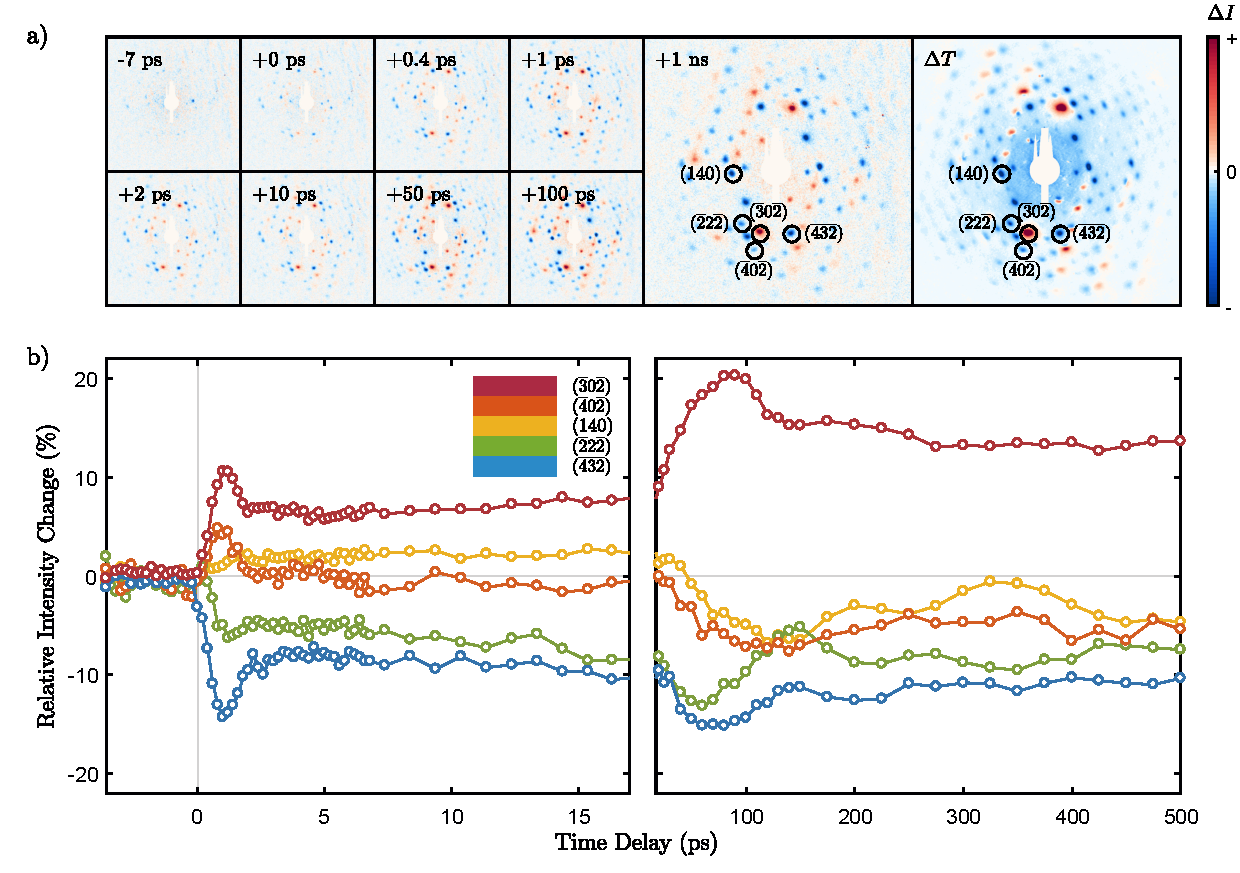
\includegraphics[width = \textwidth]{Figures/fig_EDO_TRresults.pdf}
  \caption[Time-resolved UED data of (EDO-TTF)\textsubscript{2}PF\textsubscript{6}.]{
  Time-resolved UED data of (EDO-TTF)\textsubscript{2}PF\textsubscript{6}.
  (a) Difference images at different time points show the pattern of diffraction intensity changes
  associated with the structural dynamics that follows photoexcitation of the LT ground state;
  the difference image between the LT and HT phases is included on the far right to emphasize
  the similarity between the HT diffraction pattern and that observed at $t = +1$~ns.
  (b) Time traces for some selected diffraction spots are plotted on two timescales
  (from $-3.6$ to $+17$~ps; from $+17$ to $+500$~ps)
  to showcase the presence of fast and slow processes which are at work.
  }
  \label{fig: EDO-TRresults}
\end{figure}
%
The most succinct observation is the similarity between the $+1$~ns difference image and the one measured
across the thermal phase transition, immediately suggesting that the photoinduced structural dynamics ends
at a HT-like state.

Fig.~\ref{fig: EDO-TRresults}b gives the temporal evolution of the intensity of
some selected diffraction spots. From these time traces, two components is resolved:
a `fast' change on the order of a few picoseconds and a `slow' one that proceeds on the 100-ps timescale.
%
The former can be explained as the result of femtosecond optical excitation
altering the charge distribution within the EDO-TTF stack, modifying various intermolecular and intramolecular forces,
and driving coherent molecular motions.
%
The slow component is attributed to uncorrelated motions that provide an ensemble-averaged picture
of the structural evolution, i.e.~a thermal relaxation process that brings the molecular system
to the final HT-like state~\cite{Fukazawa2012}.
%
In addition, oscillations with a period of a few hundred picoseconds are apparent after $+100$~ps
(right side of Fig.~\ref{fig: EDO-TRresults}b);
they are likely a manifestation of the transfer of heat to the lattice
as strain waves are generated~\cite{Harb2009, Maher-thesis}.
%
Finally, a plateau can be readily seen on the ultrafast timescale (left side of Fig.~\ref{fig: EDO-TRresults}b)
wherein the intensity of all diffraction spots remains unchanging over time delays between $+3$ and $+10$~ps.
This behaviour indicates the presence of a transient intermediate state~(TIS)
along the pathway of the PIPT process.
Given that optical studies give evidence to large charge fluctuations
prevailing in this time span~\cite{Onda2008, Fukazawa2012},
it is plausible that the effective intermolecular forces are screened and
the structure of the molecular system is therefore transiently locked.

To obtain a time-dependent map of the relevant molecular motions driving
the IM~phase transition and the intervening formation of the TIS structure,
a structural refinement scheme based on a parameterized molecular model is employed.
The details of this general method are described in Sec.~\ref{sec: UED-data-analysis-3}
and it is applied to (EDO-TTF)\textsubscript{2}PF\textsubscript{6} as follows.

% Spot restriction and molecular model
The set of diffraction spots used in the refinement calculations is restricted to those
which are proximate to the Ewald sphere and do not contain contribution from multiple relrods.
%
In addition, the end-point crystal structures of the linear interpolation in Eq.~\eqref{eq: linear-model}
are chosen to be those of the LT and HT phases respectively.
%
To construct the candidate structures for the time-dependent optimization,
inversion symmetry is assumed to be conserved and
the two (EDO-TTF)\textsubscript{2}PF\textsubscript{6} molecules in the unit cell
are divided by symmetric nonequivalency into three dynamical groups which display distinct motions.
%
As seen in Fig.~\ref{fig: EDO-movie}a,
the first group ($\xi_1$) is composed of atoms of the bent neutral EDO-TTF molecules
whose IM~displacement $\Delta \bscriptr_{i} = \bscriptr_{i, \text{HT}} - \bscriptr_{i, \text{LT}}$
is primarily a flattening motion;
%
the second group ($\xi_2$), the atoms of the PF\textsubscript{6} counterions that rotate and
move to the nearest point of symmetry;
%
the last group ($\xi_3$), the atoms of the flat monovalent EDO-TTF molecules
which slide perpendicularly to the stacking axis
and become translationally equivalent to the atoms of the first group;
%
\begin{figure}[ht!]
  \centering
  \includegraphics[width = \textwidth]{Figures/fig_EDO_movie.pdf}
  \caption[Structural dynamics of (EDO-TTF)\textsubscript{2}PF\textsubscript{6} in configuration space.]{
  Structural dynamics of (EDO-TTF)\textsubscript{2}PF\textsubscript{6} in configuration space.
  Refinement of the UED data is performed by
  (a) partitioning the atoms of the unit cell into three dynamical groups (highlighted in magenta, cyan, and green) and
  (b) optimizing the goodness-of-fit $P$ between the measured structural factors and the simulated ones
  over the associated reaction coordinates $\xi_1, \xi_2, \xi_3$ for each time point $t$
  (lines shown are the multiexponential fits).
  The result is (c) a reaction pathway through configuration space that fully maps
  the molecular displacements of (EDO-TTF)\textsubscript{2}PF\textsubscript{6}
  as it goes from (d) the LT state to TIS and finally a HT-like state
  (coloured respectively in blue, green, and red).
  %
  Circles are the independently optimized structures;
  the solid lines are the multiexponential fits; the dashed line is a two-dimensional projection.
  Panel (a) is courtesy of Dr.~Alexander Marx.
  }
  \label{fig: EDO-movie}
\end{figure}
%
This approach reduces the structure refinement of each pattern of diffraction intensity changes
from a problem with $3N_\text{at} - 6$ variables to one with only $3$
while still capturing most of the physics without nonsensical results caused by overfitting.

% Excitation fraction
To determine the value of the excitation fraction~$\eta_\text{exc}$
(the fraction of unit cells engaging in the PIPT process),
it is assumed that the photoexcited molecular system has fully thermalized into a HT-like state
by $t = +1$~ns and little residual thermal stress remains;
Since $F_\text{on}(\infty, \boldsymbol{q}) \approx F_\text{on}(+1 \text{ ns})$,
$\eta_\text{exc}$ is calculated to be about $10.3$~\% using Eq.~\eqref{eq: nexc},
i.e.~the equation of Coppens et~al in the low-excitation limit~\cite{CoppensBook, Coppens1998, Coppens2005}.
%
These are fair assumptions to be made here, considering that the acoustic oscillations have damped away by $t > +500$~ps,
the estimated temperature increase is less than $50$~K, and the effect of residual stress is minimized
for reflections satisfying the Laue-Bragg condition~\cite{Harb2009}.
%
Also, from optical reflectivity and in situ optical transmission measurements,
a similar value (ca.~$8$~\%) is estimated using Eq.~\eqref{eq: nexc-optical}
for the fraction of ground unit cells which are photoexcited by the pump laser pulse.
%
Furthermore, optimization of the goodness-of-fit~$P$ as a function of $\eta_\text{exc}$ and
time delay~$t$ during the structural refinement process shows a maximum of ca.~$10$~\%
that persists over the interval of 0 to $+10$~ps.
%
Given the consistency of these independent evaluations of $\eta_\text{exc}$,
it is clear that the initial excitonic correlation length only extends over about one LT unit cell
and only local structural changes are promoted with a photoconversion efficiency of about unity.
%
This result runs counter to the observation of highly cooperative `photo-domino effect' by
Chollet et~al~\cite{Chollet2004} wherein an excitation fraction of $0.7$~\%
(one absorbed photons for every 142 LT unit cells) supposedly lead to the IM~conversion fraction of $50$~\% and
a photoconversion efficiency of 71 times unity.
%
Onda et~al~\cite{Onda2014} states that the discrepancy is explained by
the incorrect assumption in the latter work that the IM~conversion fraction can be simply and directly estimated by
the change in the reflectivity of the CT2 band at $t = +3$~ps.

In Fig.~\ref{fig: EDO-movie}b, the result of the structure refinement is shown.
For each time delay $t$, a set of optimized reaction coordinates $(\xi_1, \xi_2, \xi_3)$ is obtained;
each coordinate can then be fitted by a multiexponential function
that is based on the three-level rate model
proposed by Fukazawa et~al~\cite{Fukazawa2012}:
%
\begin{equation}
  \begin{aligned}
    f(t) & =
      \left[ H(t) \left(
        c_1 \left( \mathrm{e}^{-k_2 t} - \mathrm{e}^{-k_1 t} \right) +
        c_2 \left( \mathrm{e}^{-k_4 t} - \mathrm{e}^{-k_3 t} \right) +
        c_3 \left( 1 - \mathrm{e}^{-k_5 t} \right)
        \right) \right] \ast \text{IRF}(t)
  \end{aligned}
\end{equation}
%
where $H(t)$ is the Heaviside function,
$\textrm{IRF}(t) = \mathrm{e}^{- \frac{1}{2} t^2/\tau_\text{IRF}^2}$ is
the instrument response function with $\tau_\text{IRF}$ = $430$~fs, and
$k_i, c_j$ are the time constants and coefficients to be fitted.

Altogether, the fit results are shown in Tab.~\ref{tab: EDO-fit} and
a trajectory in $\boldsymbol{\xi}$-space can be plotted that represents the reaction pathway
taken by the molecular system following photoexcitation (see Fig.~\ref{fig: EDO-movie}c).
%
\begin{table}[ht!]
  \centering
  {\renewcommand{\arraystretch}{1.5}
  \begin{tabular}{ c c c c c c c c c }
    \toprule
      & $c_1$ & $c_2$ & $c_3$ & $\tau_{1}$ (ps) & $\tau_{2}$ (ps) & $\tau_{3}$ (ps) & $\tau_{4}$ (ps) & $\tau_{5}$ (ps) \\
    \midrule
    $\xi_1 (t)$ & $15.3$ & $6.9$ & $1.46$ & $0.70$ & $0.70$ & $3.4$ & $3.6$ & $100$\\
    $\xi_2 (t)$ & $56.0$ & $1.0$ & $0.95$ & $0.49$ & $0.53$ & $2.8$ & $3.2$ & $23$\\
    $\xi_3 (t)$ & $32.0$ & $6.0$ & $1.23$ & $0.44$ & $0.45$ & $2.0$ & $4.3$ & $28$\\
    \bottomrule
  \end{tabular}
  }
  \caption{Values of the multiexponential model fitted for
  the reaction coordinates~$\xi_i$ of (EDO-TTF)\textsubscript{2}PF\textsubscript{6}.}
  \label{tab: EDO-fit}
\end{table}
%
It can be clearly seen that
the structure of (EDO-TTF)\textsubscript{2}PF\textsubscript{6} evolves from the  LT state
($\boldsymbol{\xi}(t = 0) = (0, 0, 0)$) through concerted atomic motions
towards the HT state ($\boldsymbol{\xi}(t > +100 \text{ ps}) = (1, 1, 1)$)
with a brief, few-picosecond pit stop at the TIS
($\boldsymbol{\xi}(t \sim +3 \text{ ps}) = (0.15, 0.38, 0.40)$).
%
From the relative values and timing of the reaction coordinates,
it is observed that the motions of the flat monovalent EDO-TTF molecules and
the PF\textsubscript{6} counterions are correlated.
This suggests that optical excitation mostly drives the formation of the TIS through these modes
while the bent neutral donor molecules are unchanged.
%
Furthermore, the overshooting of these two coordinates at $t = +1$~ps is indicative
of an overdamped half-cycle motion.
%
These time-dependent correlations,
in addition to the close proximity of the counterions to the charged donors,
provide evidence for the role of steric effects --- short-range repulsive interactions ---
are also important in the crystalline order and positioning of the molecules.


\subsection{Summary and Conclusions}

From Onda et~al~\cite{Onda2008},
the ex-PHH model (see App.~\ref{ap: exPHH})
can reproduce the spectral signature of the $(0101)$ excited state
by including off-site Coulomb repulsion and electron-phonon interactions that
modulate the site energies via anion displacements.
%
The UED results herein support this description and correspondingly indicate that
the motion of the PF\textsubscript{6} counterions is an important component in the evolution of
the electronically excited LT and the formation of the TIS structures.
%
This is a curious development given that
PF\textsubscript{6}$^-$ is mostly known for its chemical stability and weak coordinating ability~\cite{Strauss1993}
and its intended role in (EDO-TTF)\textsubscript{2}PF\textsubscript{6}
probably was to electrically balance the positive charges and
passively spectate the physics of the molecular system.
%
Indeed, this connection between the counterions and the charge fluctuations leading to PIPT
suggests that they ought to be targeted for chemical modification
if the electronic properties of this crystal are to be taken controlled.
%
This approach to molecular design would be similar to the anion substitution in (TMTSF)\textsubscript{2}X
that led to the synthesis of the first ambient-pressure
organic superconductor~\cite{Bechgaard1980, Bechgaard1981}.
%
In contrast, the small relative amplitude of the flattening of the neutral EDO-TTF molecules
in the formation of the TIS questions the relevance of the simple bending--flattening type
of distortion mode to the charge disproportionation.
%
Future UED experiments can focus on different sample orientations with improved spatial resolution
and apply more general refinement methods for real-space reconstruction;
ab initio electronic calculations would link the resolved dynamics of the molecular structure with
the evolution of the charge distribution.


\section{Counterion Effect in (EDO-TTF)\textsubscript{2}SbF\textsubscript{6}}
\label{sec: UED-EDOSbF6}

\begin{figure}[ht!]
  \centering
  \includegraphics[width = \textwidth]{Figures/fig_EDOSb_sample.pdf}
  \caption[Overview of (EDO-TTF)\textsubscript{2}SbF\textsubscript{6}.]{
  Overview of (EDO-TTF)\textsubscript{2}SbF\textsubscript{6}.
  (a) (EDO-TTF)\textsubscript{2}PF\textsubscript{6} and (EDO-TTF)\textsubscript{2}SbF\textsubscript{6}
  are isostructural in both LT and HT phases.
  (b) All three hexafluoropnictate derivatives of (EDO-TTF)\textsubscript{2}X
  exhibit similar MI~phase transitions but with decreasing $T_\text{MI}$ and
  increasing $\Delta T_\text{MI}$ for larger counterions.
  (c) Black (EDO-TTF)\textsubscript{2}SbF\textsubscript{6} crystals
  in a sample vial, next to   a block of epoxy resin with a singular crystal embedded
  on top in preparation for ultramicrotomy.
  Panel~(b) is adapted from Ref.~\cite{NakanoX} with permission
  from Prof.~Yoshiaki Nakano.
  }
  \label{fig: EDOSb-sample}
\end{figure}

Bechgaard-Fabre salts mostly assemble into similar crystal structures and
showcase a similar procession of ground states and collective phenomena
as different anions are substituted (see Fig.~\ref{fig: EDO-overview}d).
%
In particular, molecules of the (EDO-TTF)\textsubscript{2}X where X is one of the hexafluoropnictates
form isostructural crystals (Fig.~\ref{fig: EDOSb-sample}a) and
exhibit the same type of thermal MI~phase transition~\cite{Ota2002, Ota2003, Nakano2009}.
%
As seen in Fig.~\ref{fig: EDOSb-sample}b,
this phase transition is manifested by a sudden change in magnetic susceptibility of the material
as the Pauli paramagnetism%
\footnote{Named for Wolfgang Pauli (1900--1958) and his eponymous exclusion principle,
Pauli paramagnetism refers to the tendency of a `metal' to become weakly magnetized
under an applied magnetic field as its free electrons align with the field~\cite{Nobel1942, AshcroftBook}.}
of the metallic phase disappears in the insulator phase.

The parameters of the thermal MI~phase transition down this chemical series
are tabulated in Tab.~\ref{tab: EDO-TMI}.
Two trends can be seen as the size of the substituted pnictogen is increased:
a lowering of the transition temperature $T_\text{MI}$ and
a widening of the hysteresis loop $\Delta T_\text{MI}$~\cite{NakanoX}.
%
This observation, in addition to later work by Ota et~al~\cite{Ota2006}
where X is replaced by even larger anions ($\mathrm{GaCl_4^-}$ and $\mathrm{ReO_4^-}$),
suggests that large counterions can penetrate the EDO-TTF stack and
affect the electronic correlation relevant to the MI~phase transition.

Furthermore, it has been found spectroscopically that
the reverse insulator--metal phase transition can be triggered on the ultrafast timescale
in (EDO-TTF)\textsubscript{2}PF\textsubscript{6} by photoexcitation of
one of its charge-transfer bands~\cite{Chollet2004, Onda2008, Fukazawa2012}.
%
In the UED work described in Sec.~\ref{sec: UED-EDOPF6},
it has also been shown that the motion of the PF\textsubscript{6} counterions
plays a critical role in enabling this IM~transition by allowing the EDO-TTF molecules
to approach each other and interact, leading to the IM~transition.
%
However, no such PIPT could be detect in crystals of
(EDO-TTF)\textsubscript{2}SbF\textsubscript{6}~\cite{Lorenc2008, Servol2015}.
Time-resolved measurements of photoinduced changes in reflectivity only reveal
the excitation of some optical phonons followed by the formation of a local state
similar to the TIS of the PF\textsubscript{6} derivative, tentatively suggesting
that the larger counterion increases the distance between the EDO-TTF molecules
--- thus the unit-cell volume change~$\frac{\Delta V}{V_\text{HT}}$ (Tab.~\ref{tab: EDO-TMI})
and the resulting elastic energy cost necessary for the IM~transition ---
beyond what can be achieved during the photoinduced process~\cite{Servol2015}.
More details could be found in the doctoral theses in Refs.~\cite{Moisan-thesis, Kaszub-thesis}.

Therefore, a UED study on (EDO-TTF)\textsubscript{2}SbF\textsubscript{6} is called for
to follow-up on the previous work in Sec.~\ref{sec: UED-EDOPF6} and
offer direct structural confirmation of this `counterion effect.'
The resulting work is described as follows.

\begin{table}[ht!]
  \centering
    \begin{tabular}{c c c c c c}
      \toprule
      X & $T_{\text{MI}\downarrow}$~(K) & $T_{\text{MI}\uparrow}$~(K) & $T_\text{MI}$~(K) & $\Delta T_\text{MI}$~(K) & $\Delta V / V_\text{HT}$~(\%) \\
      \midrule
      PF\textsubscript{6}  & 278.5 & 279.5 & 279.0 & 1.0  & $-0.45$ \\
      AsF\textsubscript{6} & 268.0 & 273.5 & 270.8 & 5.5  & $-0.77$ \\
      SbF\textsubscript{6} & 235.0 & 249.0 & 242.0 & 14.0 & $-1.39$ \\
      \bottomrule
    \end{tabular}
  \caption{Hysteresis of the thermal MI~phase transition of different (EDO-TTF)\textsubscript{2}X.
    $T_{\text{MI}\downarrow}$ and $T_{\text{MI}\uparrow}$ are the transition temperature
    during the cooling and heating cycles respectively;
    $T_\text{MI} = \frac{1}{2} (T_{\text{MI}\downarrow} + T_{\text{MI}\uparrow})$ and
    $\Delta T_\text{MI} = T_{\text{MI}\uparrow} - T_{\text{MI}\downarrow}$.
    $\Delta V / V_\text{HT}$, where $\Delta V = V_\text{LT} - V_\text{HT}$,
    is the associated relative change in unit-cell volume at $T_\text{MI}$.
    The values herein are courtesy of Prof.~Yoshiaki Nakano~\cite{Nakano2008, NakanoX}.}
  \label{tab: EDO-TMI}
\end{table}

\subsection{Methods}

Single-crystals of (EDO-TTF)\textsubscript{2}SbF\textsubscript{6} are synthesized in
an analoguous manner as those of (EDO-TTF)\textsubscript{2}PF\textsubscript{6}
--- by electrocrystallization in ethanol.
The supporting electrolyte employed here is freshly purified (Bu\textsubscript{4}N)SbF\textsubscript{6}
whereas the original method used (EMI)SbF\textsubscript{6}
(EMI refers to 1-ethyl-3-methylimidazolium)~\cite{Maesato2009}.
%
These resulting dark crystals (see Fig.~\ref{fig: EDOSb-sample}c) are mounted on epoxy resin and
cleaved by ultramicrotomy into slices that are $150$~nm thick and typically $500$~$\unslant\mu$m across.
They are then scooped onto copper TEM meshes and mounted in the UED sample chamber.
%
During the UED measurements, the samples are kept at $180$~K using the liquid nitrogen cold finger,
well below the hysteresis loop of the MI~phase transition as seen in Fig.~\ref{fig: EDOSb-sample}b,
to ensure that they are fully in the LT phase ($T_\text{MI} = 242$~K and $\Delta T_\text{MI} = 14$~K).

The UED setup used herein is the same as the one in Sec.~\ref{sec: UED-EDOPF6} and
it is described in detail in Sec.~\ref{sec: UED-setup}.
%
In particular, the electron pulse duration is measured to be ca.~$300$~fs FWHM~\cite{Gao2013b}.
The pump laser has pulse duration of $60$~fs, centre wavelength of $800$~nm, and
a polarization that is adjusted to maximize sample absorption via the CT2 band.
The laser repetition rate is set at $10$~Hz to avoid damage of the sample caused by
cumulative heating.
%
At the sample position, the laser pulse energy is $0.63$~mJ/cm$^2$.
The excitation fraction $\eta_\text{exc}$ is determined to be ca.~$10$~\%
using the methods described in Sec.~\ref{sec: UED-EDO-Results}.

For data analysis, an approach different to that used for (EDO-TTF)\textsubscript{2}PF\textsubscript{6}
is adopted. By considering the similarity between broadband TA spectra and
time-resolved electron diffraction data, this work marks the first application of the SVD-based method described
in Sec.~\ref{sec: UED-data-analysis-2}.


\subsection{Experimental Results and Discussions}

\begin{figure}[ht!]
  \centering
  \includegraphics[width = \textwidth]{Figures/fig_EDOSb_UEDimages.pdf}
  \caption[Static and time-resolved electron diffraction patterns of
    (EDO-TTF)\textsubscript{2}SbF\textsubscript{6}.]{
    Electron diffraction patterns of (EDO-TTF)\textsubscript{2}SbF\textsubscript{6}:
    (a) static image of the LT phase ($T = 170$~K) with select spots circled for later reference;
    (b) difference image between the HT ($T = 300$~K) and LT phase;
    (c) scatter plot of the integrated intensity in Panel~(b);
    (d) scatter plot of the integrated intensity of the time-resolved difference image at $t = +100$~ps.
    %
    The size of the markers in Panels~(c) and (d) scales with the intensity of the diffraction spots
    and the face colour scales with the intensity difference.
  }
  \label{fig: EDOSb-UEDimages}
\end{figure}

The panels of Fig.~\ref{fig: EDOSb-UEDimages} show the electron diffraction patterns
of the (EDO-TTF)\textsubscript{2}SbF\textsubscript{6} samples in different states for comparison.
%
In Panel~(a), data for the LT phase is shown and a large number of diffraction spots can be seen.
They range from peaks close to the (000) transmitted beam to the high-order ones
near the edge of the camera sensor, suggesting a high degree of sample crystallinity and
a transverse beam coherence that is on the order of a few nanometers and thus sufficient to
atomically resolved changes to the crystal structure.

In Panel~(b), the difference image between the LT data and that collected when the sample is in
the HT phase ($T = 300$~K) is shown. Red and blue patches indicate the pattern of diffraction spots
that have respectively increased and decreased in intensity and/or have shifted in position within
reciprocal space. The former type of intensity changes is generally caused by atomic motions;
the latter would be associated with distortions in the shape or size of the unit cell.
Using the scattering equations described in Sec.~\ref{sec: UED-physics} and
refined HT and LT crystal information from Nakano et~al~\cite{NakanoX},
it is found that the observed thermal difference image is consistent with
the structural reorganization correlated with the MI~phase transition
of (EDO-TTF)\textsubscript{2}SbF\textsubscript{6}.

The scatter plots in Panels~(c) and (d) represent a reconstructed diffraction pattern where each marker
is sized and coloured respectively according to the diffraction spot intensity in the LT phase and
the relative change in intensity. As described in Sec.~\ref{sec: UED-data-analysis-1},
the position of the spots is fitted using Eq.~\eqref{eq: gaussian-spot} and
the intensity is calculated by integrating the detector counts in a circular region around the spot position.
%
In particular, Panel~(c) shows the changes in spot intensity that are caused by
the thermal IM~phase transition, and Panel~(d),
those that occur $100$~ps after photoexcitation of the CT2 band.
Clearly, the patterns do not match, thus indicating that the late-time molecular structure of
the photoinduced state of (EDO-TTF)\textsubscript{2}SbF\textsubscript{6} is not the same as
the structure of both the LT and HT states.
Furthermore, there is no discernible change in the position of the diffraction spots,
which is unsurprising since volume expansion of the unit cell is not expected
so soon after photoexcitation~\cite{Lorenc2009}
nor large enough to be resolvable presently~\cite{Gao2013}.

In Fig.~\ref{fig: EDOSb-UEDtraces}, the ultrafast structural dynamics
of both PF\textsubscript{6} and SbF\textsubscript{6} derivatives are compared.
%
The time traces for a number of diffraction spots are shown in Panels~(a) and (b);
these precise spots are selected to highlight the diversity of signals that can be
observed amongst the hundreds of features in the time-resolved diffraction patterns.
%
In particular, the PF\textsubscript{6} data is characterized by an sub-picosecond peak
that is followed by a few-picosecond plateau and then a slow evolution towards a HT-like state;
the Sb\textsubscript{6} data only shows bi-exponential dynamics on the order of tens of picoseconds
that terminates at a state structurally unlike either thermally accessible states.
%
Indeed, counterion substitution has a significant effect on the ultrafast structural reorganization
that occurs following photoexcitation.
%
\begin{figure}[ht!]
  \centering
  \includegraphics[width = \textwidth]{Figures/fig_EDOSb_UEDtraces.pdf}
  \caption[Time-resolved UED data of (EDO-TTF)\textsubscript{2}X
    (X = PF\textsubscript{6}, SbF\textsubscript{6}).]{
    Time-resolved UED data of (EDO-TTF)\textsubscript{2}X,
    where X = PF\textsubscript{6} (left panels) and SbF\textsubscript{6} (right panels).
    The top panels, (a) and (b), show the relative change in diffraction intensity
    at select diffraction spots following photoexcitation.
    The bottom panels, (c) and (d), show the principal right-singular vectors
    of the UED data; the insets are plots of $\log_{10} s_i$, where $s_i$ are the singular values
    sorted in descending order.
    The markers are measured values and the solid lines are lines of best fit
    from a global analysis.
  }
  \label{fig: EDOSb-UEDtraces}
\end{figure}

To better elucidate the influence of the counterion in the processes that could lead to PIPT,
a more sophisticated data analysis approach is necessary.
Previous UED works involved a mapping from reciprocal to real space;
a purpose-built structure model is refined against each time-resolved diffraction pattern
in the image stack to get a set of time-dependent reaction coordinates.
Here, the projection of the structural dynamics is performed instead
directly from within reciprocal space.
%
This is possible since the number of observable diffraction spots (ca.~$200$ Friedel pairs)
is greater than the number of possible degrees of freedom~(DOFs) available to (EDO-TTF)\textsubscript{2}X
($N_\text{at} = 35$ non-hydrogen atoms in the asymmetric unit; $3 N_\text{at} - 6 = 99$~DOFs).
A similar oversampling situation exists in broadband TA spectroscopy,
wherein the number of probed wavelengths is much greater than
the number of optically active species within the probe volume.
%
Then, it follows that singular value decomposition~(SVD) can be applied
to reduce the amount of redundant complexity in the measured dataset.

As described in Sec.~\ref{sec: UED-data-analysis-2},
SVD is a generalization of eigenvalue decomposition to any non-square $m \times n$~matrix;
it factorizes the matrix into three parts:
a $M \times N$ diagonal matrix whose diagonal elements are the `singular values' and
two orthogonal matrices on the left ($M \times M$) and right ($N \times N$)
whose columns are respectively the `left-' and `right-singular vectors'.
%
In application to UED data, the matrix to be factorized is simply the column-wise concatenation
of the time traces where $M$ is the number of diffraction spots and $N$ is the number of time points;
the resulting factors then form orthogonal basis sets that fully span their respectively spaces:
the left-singular vectors for the reciprocal space domain and the right-singular vectors for the time domain.
Since reciprocal space is dual to real space, the basis vectors of the former simply represent
orthogonal sets of atomic motions or `molecular modes.'
%
Furthermore, it is observed that not all the vectors of these basis sets contribute equally.
The insets of the bottom panels of Fig.~\ref{fig: EDOSb-UEDtraces} show logarithmic plots
of the singular values sorted in descending order for the PF\textsubscript{6} and SbF\textsubscript{6} datasets:
only the first few values are significant while the rest are effectively zero
and there is a clear point of flexion in the trendline.
%
A low-rank approximation can then be applied by keeping only the principal components
and neglecting the rest.
%
In the case of X = PF\textsubscript{6}, there are three principal components (Fig.~\ref{fig: EDOSb-UEDtraces}c);
in the case of X = SbF\textsubscript{6}, there are only two (Fig.~\ref{fig: EDOSb-UEDtraces}d).
%
This suggests that the atomic motions activated by the photoexcitation of either molecular system
live in a much lower dimensional space than what their respective degrees of freedom
would have otherwise indicated.
%
This insight thus furthers and sets the present work apart from others,
such as Schmidt et~al~\cite{Schmidt2003} who proposed applying SVD in real space
to time-resolved XRD electron density maps as a mean to reduce the accrued random noise.

Note that the fit lines of the UED data (Panels~(a) and (b) of Fig.~\ref{fig: EDOSb-UEDtraces})
are derived from a global analysis model wherein the principal right-singular vectors are fitted
to a sum of exponential terms convolved with a Gaussian IRF (Eq.~\eqref{eq: UED-GA}).
%
The entirety of the X = PF\textsubscript{6} data is fitted with only the three principal components
and four exponential terms with time constants $\tau_1 = 0.99$~ps, $\tau_2 = 1.07$~ps, $\tau_3 = 28.01$~ps, and
$\tau_4 = 45.49$~ps.
For the X = SbF\textsubscript{6} data, the fit used the two principal components and
two exponential terms with time constants $\tau_1 = 25.23$~ps and $\tau_2 = 51.65$~ps.
%
No decay- or species-associated traces are shown since UED is structural probe of
locally excited molecules, not uniquely associated populations of excited states which follow
photochemical kinetics.

To build on the results of the SVD analysis, a Pearson correlation analysis is performed.
As in Eq.~\eqref{eq: UED-Pearson}, the Pearson correlation coefficients between
the time-dependent structure factors of the photoexcited state and
the static ones of the thermal equilibrium states are calculated.
The resulting values form a set of coordinates $\boldsymbol{P}(t) = \left( P_\text{exc, HT}(t), P_\text{exc, LT}(t) \right)$
in a configuration subspace spanned by the LT and HT structures.
%
In Fig.~\ref{fig: EDOSb-Pearson}, these points trace out a trajectory that shows
the time evolution of the structure of the photoexcited (EDO-TTF)\textsubscript{2}X
relative to their known structures, normalized to ensure that
$(0, 1)$ and $(1, 0)$ specify the LT and HT structures respectively.
%
\begin{figure}[ht!]
  \centering
  \includegraphics[width = \textwidth]{Figures/fig_EDOSb_Pearson.pdf}
  \caption[Time-dependent Pearson correlation of (EDO-TTF)\textsubscript{2}X
    (X = PF\textsubscript{6}, SbF\textsubscript{6}).]{
    Time-dependent Pearson correlation of the UED data of (EDO-TTF)\textsubscript{2}X,
    where X = (a) PF\textsubscript{6} and (b) SbF\textsubscript{6}.
    %
    For each time delay $t$, the correlation between the measured diffraction pattern of
    the photoexcited state and either equilibrium states is calculated
    ($P = 0$, no correlation; $P = 1$, perfect correlation).
    The thick line is a trajectory that is calculated
    using the fitted, interpolated UED intensities from global analysis;
    the thin line is the two-dimensional projection of the trajectory.
    Regions associated with the structures of identifiable states are labeled by colour.
  }
  \label{fig: EDOSb-Pearson}
\end{figure}
%
For $t < 0$~ps, both molecules are in the LT ground state at $(0, 1)$.
After $t = 0$~ps, they are photoexcited and the trajectories start to diverge from each other.
%
In Panel~(a), it can be seen that the structure of the (EDO-TTF)\textsubscript{2}PF\textsubscript{6} molecule
moves rapidly towards the HT state, overshoots, settles in the TIS at $(0.3, 0.9)$
for a few picoseconds, then finally relaxes to the final HT-like state.
%
On the other hand, in Panel~(b), the photoexcited structure of the X = SbF\textsubscript{6} derivative
evolves away from the structure of both the LT and HT states on a timescale of several tens of picoseconds,
bypassing the region of configuration space where its equivalent TIS structure would exist.
%
Indeed, the marked difference in shape of the two configuration trajectories
in Fig.~\ref{fig: EDOSb-Pearson} highlights the important role played by the counterion
in the PIPT of the (EDO-TTF)\textsubscript{2}X molecular system.

The earlier UED work on the X = PF\textsubscript{6} derivative
identified the three independent atomic motions that comprise the basis set for
fully describing the overall structural dynamics, one of these being the counterion motion
which is correlated with the formation of the TIS.
%
The present work recovers these modes in the form of the three principal components from the SVD analysis.
This suggests that the missing third mode in the X = SbF\textsubscript{6} UED data is
the counterion motion which would have steered its Pearson trajectory through the equivalent TIS region
in configuration space.
%
Thus, in a manner consistent with the proposed mechanism of Servol et~al~\cite{Servol2015},
the deactivation of the photoinduced IM~pathway in (EDO-TTF)\textsubscript{2}SbF\textsubscript{6} can be
explained by the conspicuous absence of this key mode.

Although the counterions are not directly involved in the photophysical process,
they play a crucial role in passively guided structural reorganization of the photoexcited cations.
This observation can be rationalized when the change in the local electric field due to
the photoinduced electron transfer between EDO-TTF molecules is considered.
%
In this view, the counterions move simply in response of the electrostatic reaction forces
and end up directing the lattice reorganization that destabilizes the charge-ordered state of the LT phase.
This motion is thus intimately coupled to the collective lattice response to photoexcitation
and the resulting change in material properties during PIPT.
In corollary, larger counterions would be too sterically encumbered to move accordingly,
preventing PIPT in isostructural derivatives of (EDO-TTF)\textsubscript{2}PF\textsubscript{6}
further down the chemical series. If the volume of the photoexcited LT unit cell could expand
on the ultrafast timescale and reduce steric hindrance, then this counterion effect may be less pronounced.

Fukazawa et~al also studied in their work~\cite{Fukazawa2013} the effect of counterion size
using time-resolved IR vibrational spectroscopy on the photoinduced phase transition of
another photoactive molecular system --- X[Pd(dmit)\textsubscript{2}]\textsubscript{2},
where X =  Cs and Et\textsubscript{2}Me\textsubscript{2}Sb%
\footnote{dmit = dimercaptoisotrithione or 1,3-dithiol-2-thione-4,5-dithiolate,
Et = C\textsubscript{2}H\textsubscript{5}, and Me = CH\textsubscript{3}.} ---
and observed that substitution for a larger counterion changes the order of the PIPT and
greatly delays the emergence of the final HT-like state
($\tau_\text{PIPT} = 0.1$~ps $\rightarrow 70$~ps).
%
The present UED results off the first direct structural evidence of the counterion effect
on lattice reorganization destabilizing the charge order of an insulator state and
the subsequent formation of a metallic state.
In particular, there are only a few types of atomic motions that dominate the structural transition,
as opposed to an equipartitioning to all possible degrees of freedom;
this phenomenon appears general and it is herein referred to as `dimensionality reduction'~\cite{Miller2016}.
The notion of key reaction modes has been discussed in the field of chemistry for some time;
they can now be observed directly using time-resolved structural probes like UED and
be used to explain how even a simple change in counterion can affect
the degree of lattice reorganization in charge-transfer processes and
be used to control macroscopic material properties.
%
Furthermore, this work has successfully demonstrated how SVD analysis belongs in the standard toolbox
for directly interpreting time-resolved diffraction data, without reliance on refinement models
that would map reciprocal-space features to real-space ones.

\subsection{Summary and Conclusions}

In this work, the structural dynamics of (EDO-TTF)\textsubscript{2}SbF\textsubscript{6} is
elucidated using a combination of SVD and Pearson analysis.
It is also the first comparative UED study of an isostructural family of molecules
with the goal of investigating the interplay between structural dynamics and molecular function
in close detail. The results show that the size of the counterion is a key factor for
determining the activity of the photoinduced IM~pathway and the dimensionality of
the associated atomic motions.
%
In the case of X = PF\textsubscript{6}, the structural dynamics is three-dimensional
in terms of generalized coordinates and one of three principal modes is
a counterion movement that leads to lattice relaxation and formation of the metallic state.
When X = SbF\textsubscript{6}, the dynamics becomes two-dimensional as the counterion is too large
and cannot avoid hindering the interactions between the EDO-TTF molecules;
this obstruction prevents full relaxation to the structural relationships
that enable the charge redistribution and spatial electron delocalization
necessary for the formation of a metallic band structure.
%
This conclusion is consistent with the mechanism proposed by others~\cite{Servol2015},
the interplay of cavity size and counterion size~\cite{Kistenmacher1984},
and the general sensitivity of (EDO-TTF)\textsubscript{2}X~\cite{Nakano2008, Nakano2009, NakanoX, Ishikawa2014}
and Bechgaard-Fabre salts~\cite{Kohler2011, Dressel2012, Pouget2018} to chemical and
isotope substitution.

In particular, the present work is not based on structural refinement models;
instead, it is understood using SVD in reciprocal space, an approach that has been
well-established for spectroscopic techniques involving overlapped spectra components.
Here, SVD is used as an unbiased method to analyze time-resolved diffraction data and
project out the dominant atomic motions involved in the structural dynamics.
%
There are clearly only a few key modes, greatly reducing the dimensionality of
the problem of chemistry:
the convolution of all nuclear motions possible in a reaction mechanism
to a single putative coordinate for the purpose of controlling molecular processes.
%
Indeed, these findings illustrate the great promise that the techniques used herein
bears for further application to other diffraction experiments.


% Dressel2012:
% charge disproportionation/imbalance (reflectivity) <-> vibrational modes (IR, Raman)
% larger anion -> larger intrastack distance ->? more pronounced intersite Coulomb repulsion
% anion-sulfur distance vs. charge ordering
% lattice vib. coupling modulates transfer integral, intramolecular vib. coupling modulates on-site energy
% HOMO of molecule shows charge mainly located on sulfur atoms and C=C bonds
% motion of anions slows down with low T, lock in place inside cavity (anion rotational disorder lifted) -> anion ordering <- anion-F-S long-range interaction
% charge disproportionation increases from PF6 to SbF6

% Role of cavity and anion size in TMTSF salts (1984):
% Kistenmacher, T.J. Cavity sice versus anion size in (TMTSF)2X salts - possible implications for the uniqueness of (TMTSF)2ClO4. Solid State Commun. 1984, 50, 729–733.
% Kistenmacher, T. Anion-donor coupling in (TMTSF)2X salts—Symmetry considerations. Solid State Commun. 1984, 51, 931–934.

% Deuteration modulates the electron-molecular-vibration (e-mv) coupling and
% increases the transition temperature by $3.5$~K
% Substituent effect (CLEDO-TTF and MeEDO-TTF)
